%%% LaTeX Template: Article/Thesis/etc. with colored headings and special fonts
%%%
%%% Source: http://www.howtotex.com/
%%% Feel free to distribute this template, but please keep to referal to http://www.howtotex.com/ here.
%%% February 2011
%%%
%%% Modified May 2018 by CDM

%%%  Preamble
\documentclass[11pt,letterpaper]{article}
\usepackage[margin=1.0in]{geometry}
\usepackage[T1]{fontenc}
\usepackage[bitstream-charter]{mathdesign}
\usepackage[latin1]{inputenc}					
\usepackage{amsmath}						
\usepackage{xcolor}
\usepackage{cite}
\usepackage{hyphenat}
\usepackage{graphicx}
\usepackage{float}
\usepackage{subfigure}
\usepackage{sectsty}
\usepackage[compact]{titlesec} 
\usepackage[tablegrid]{vhistory}
\allsectionsfont{\color{accentcolor}\scshape\selectfont}

%%% Definitions
\definecolor{accentcolor}{rgb}{0.0,0.0,0.5} 
\newcommand{\teamname}{Robo Crew}
\newcommand{\productname}{RV8 Workcell}
\newcommand{\coursename}{CSE 4316: Senior Design I}
\newcommand{\semester}{Fall 2023}
\newcommand{\docname}{System Requirements Specification}
\newcommand{\department}{Department of Computer Science \& Engineering}
\newcommand{\university}{The University of Texas at Arlington}
\newcommand{\authors}{Muhammad Anas \\ Ameen Mahouch \\ Akshay Paluri  \\ Hyun Ho Kim \\ Kundan Singh Mahato }

%%% Headers and footers
\usepackage{fancyhdr}
	\pagestyle{fancy}						% Enabling the custom headers/footers
\usepackage{lastpage}	
	% Header (empty)
	\lhead{}
	\chead{}
	\rhead{}
	% Footer
	\lfoot{\footnotesize \teamname \ - \semester}
	\cfoot{}
	\rfoot{\footnotesize page \thepage\ of \pageref{LastPage}}	% "Page 1 of 2"
	\renewcommand{\headrulewidth}{0.0pt}
	\renewcommand{\footrulewidth}{0.4pt}

%%% Change the abstract environment
\usepackage[runin]{abstract}			% runin option for a run-in title
%\setlength\absleftindent{30pt}			% left margin
%\setlength\absrightindent{30pt}		% right margin
\abslabeldelim{\quad}	
\setlength{\abstitleskip}{-10pt}
\renewcommand{\abstractname}{}
\renewcommand{\abstracttextfont}{\color{accentcolor} \small \slshape}	% slanted text

%%% Start of the document
\begin{document}

%%% Cover sheet
{\centering \huge \color{accentcolor} \sc \textbf{\department \\ \university} \par}
\vspace{1 in}
{\centering \huge \color{accentcolor} \sc \textbf{\docname \\ \coursename \\ \semester} \par}
\vspace{0.5 in}
\begin{figure}[h!]
	\centering
   	
\includegraphics[width=0.60\textwidth]{images/robocrew.jpg}
\end{figure}
\vspace{0.5 in}
{\centering \huge \color{accentcolor} \sc \textbf{\teamname \\ \productname} \par}
\vspace{0.5 in}
{\centering \large \sc \textbf{\authors} \par}
\newpage


%\vspace{1 in}
%\centerline{January 13th, 2012}
%\newpage

%%% Revision History
\begin{versionhistory}
  	\vhEntry{0.1}{10.16.2023}{AM, MA, HK, AP, KM}{Document Creation}
    \vhEntry{0.2}{05.05.2024}{AM, MA, HK, AP, KM}{Document Update}
\end{versionhistory}


\newpage

%%% Table of contents
\setcounter{tocdepth}{3}
\tableofcontents
\newpage

%%% List of figures and tables (optional)
\listoffigures
%\listoftables
\newpage

\section{Product Concept}
This section describes the purpose, use, and intended user audience for the RV8 Work Cell. RV8 Work Cell is a system that performs palletizing and depalletizing of boxes in an industrial manner. Users of this work cell will be able to practice standards in industrial robotics, while increasing time efficiency. 
\subsection{Purpose and Use}
The conventional approach to material handling in warehouses contains several challenges. Palletizing and depalletizing boxes manually is a time-consuming task, which decreases productivity. Moreover, manual material handling poses inherent risks to the workforce. Accidents and injuries are a constant concern, impacting both employee well-being and company reputation. Finally, with modern commerce continuing to grow, warehouses must adapt to higher volumes of goods and fulfill needs with efficiency. Manual processes often hinder the ability to meet customer demands effectively. The RV8 robot work cell will palletize and depalletize boxes in an organized manner according to customer's requirements with high efficiency and accuracy.

\subsection{Intended Audience}
This product is considered industrial, so the intended audience of this product are warehouses and factories where manual labor can be automated through the use of robotics.

\begin{figure}[h!]
	\centering
   	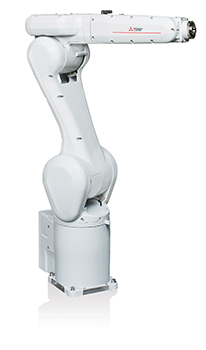
\includegraphics[width=0.40\textwidth]{images/rv8crl.jpeg}
    \caption{Mitsubishi RV8-CRL  \cite{MitsubishiRV8CRL}}
\end{figure}

\newpage
\section{Product Description}
This section provides the reader with an overview of the RV8 robot work cell. The primary operational aspects of the product, from the perspective of end users, maintainers and administrators, are defined here. The key features and functions found in the work cell, as well as critical user interactions are described in detail below.

\subsection{Features \& Functions}
The RV8 work cell will specialize in palletizing and depalletizing boxes. It will perform these operations through the use of a hydraulic gripper, vision sensors, and QR code scanners. The vertical robot initially has 6 axis, with a linear rail acting as the 7th axis. The robot will stack boxes on pallets, sorting the boxes through the use of scanner data. While performing the operation, several safety features will be implemented, such as emergency stops, industrial light towers, and presence detection within the work cell. The integrated components of the work cell are the programmable logic controller (PLC), host PC, and a CR800 handheld controller.

\subsection{External Inputs \& Outputs}
\begin{table}[H]
\resizebox{\textwidth}{!}{
\begin{tabular}{|l|l|l|l|}
\hline
 \textbf{Name} & \textbf{Description} & \textbf{Use}\\ \hline
 QR Code Scanner  & Application input & Scans the presence of boxes \\ \hline
 Presence Detection & System input & Detects motion within the work cell  \\ \hline
 Emergency Stops & User input & Stops the operation of the robot arm \\ \hline
 Industrial Light Tower  & System output & Indicates the state of the work cell  \\ \hline
 Raspberry Pi & I/O Logic & Handles the data from the QR code reader\\ \hline
\end{tabular}}
\caption{Overview of external inputs and outputs}
\end{table}

\subsection{Product Interfaces}
Specify what all operational (visible) interfaces look like to your end-user, administrator, maintainer, etc. Show sample/mocked-up screen shots, graphics of buttons, panels, etc. Refer to the critical external inputs and outputs described in the paragraph above.

\begin{figure}[h!]
	\centering
   	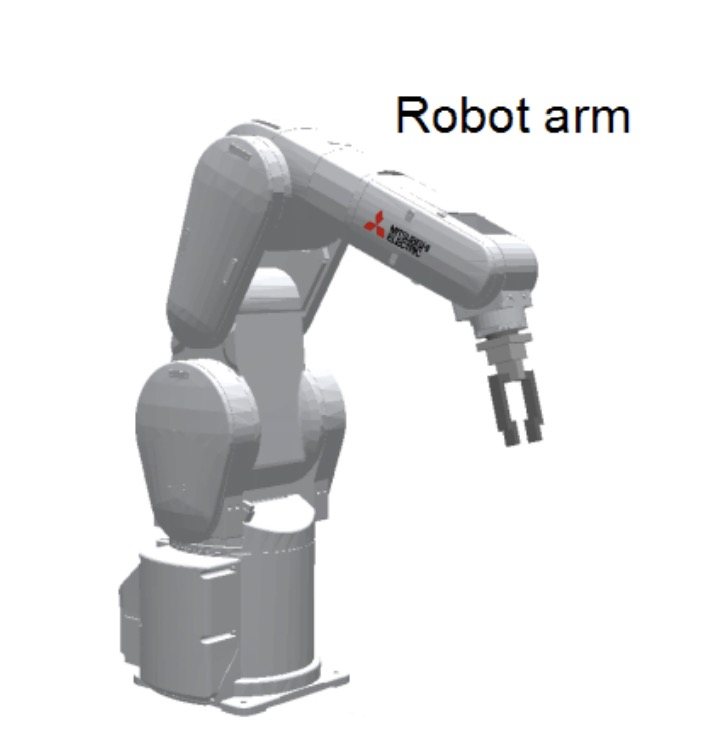
\includegraphics[width=0.30\textwidth]{images/RobotArm.jpg}
    \caption{Robot arm of RV8-CRL
    }
\end{figure}
\begin{figure}[h!]
	\centering
   	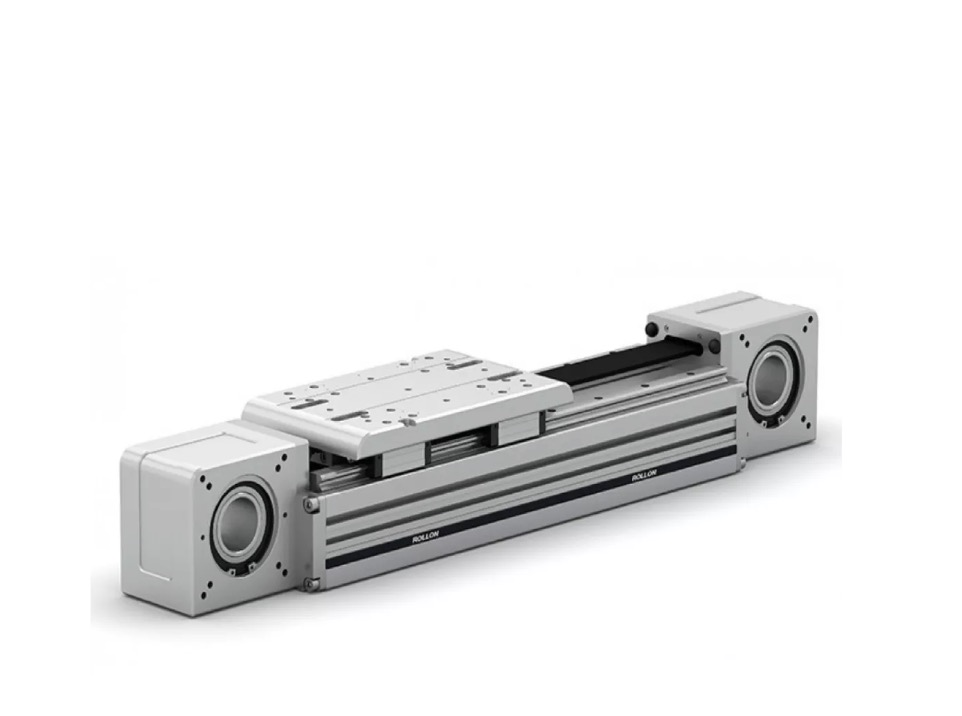
\includegraphics[width=0.40\textwidth]{images/LinearRail.jpg}
    \caption{Linear rail}
\end{figure}

\begin{figure}[h!]
	\centering
   	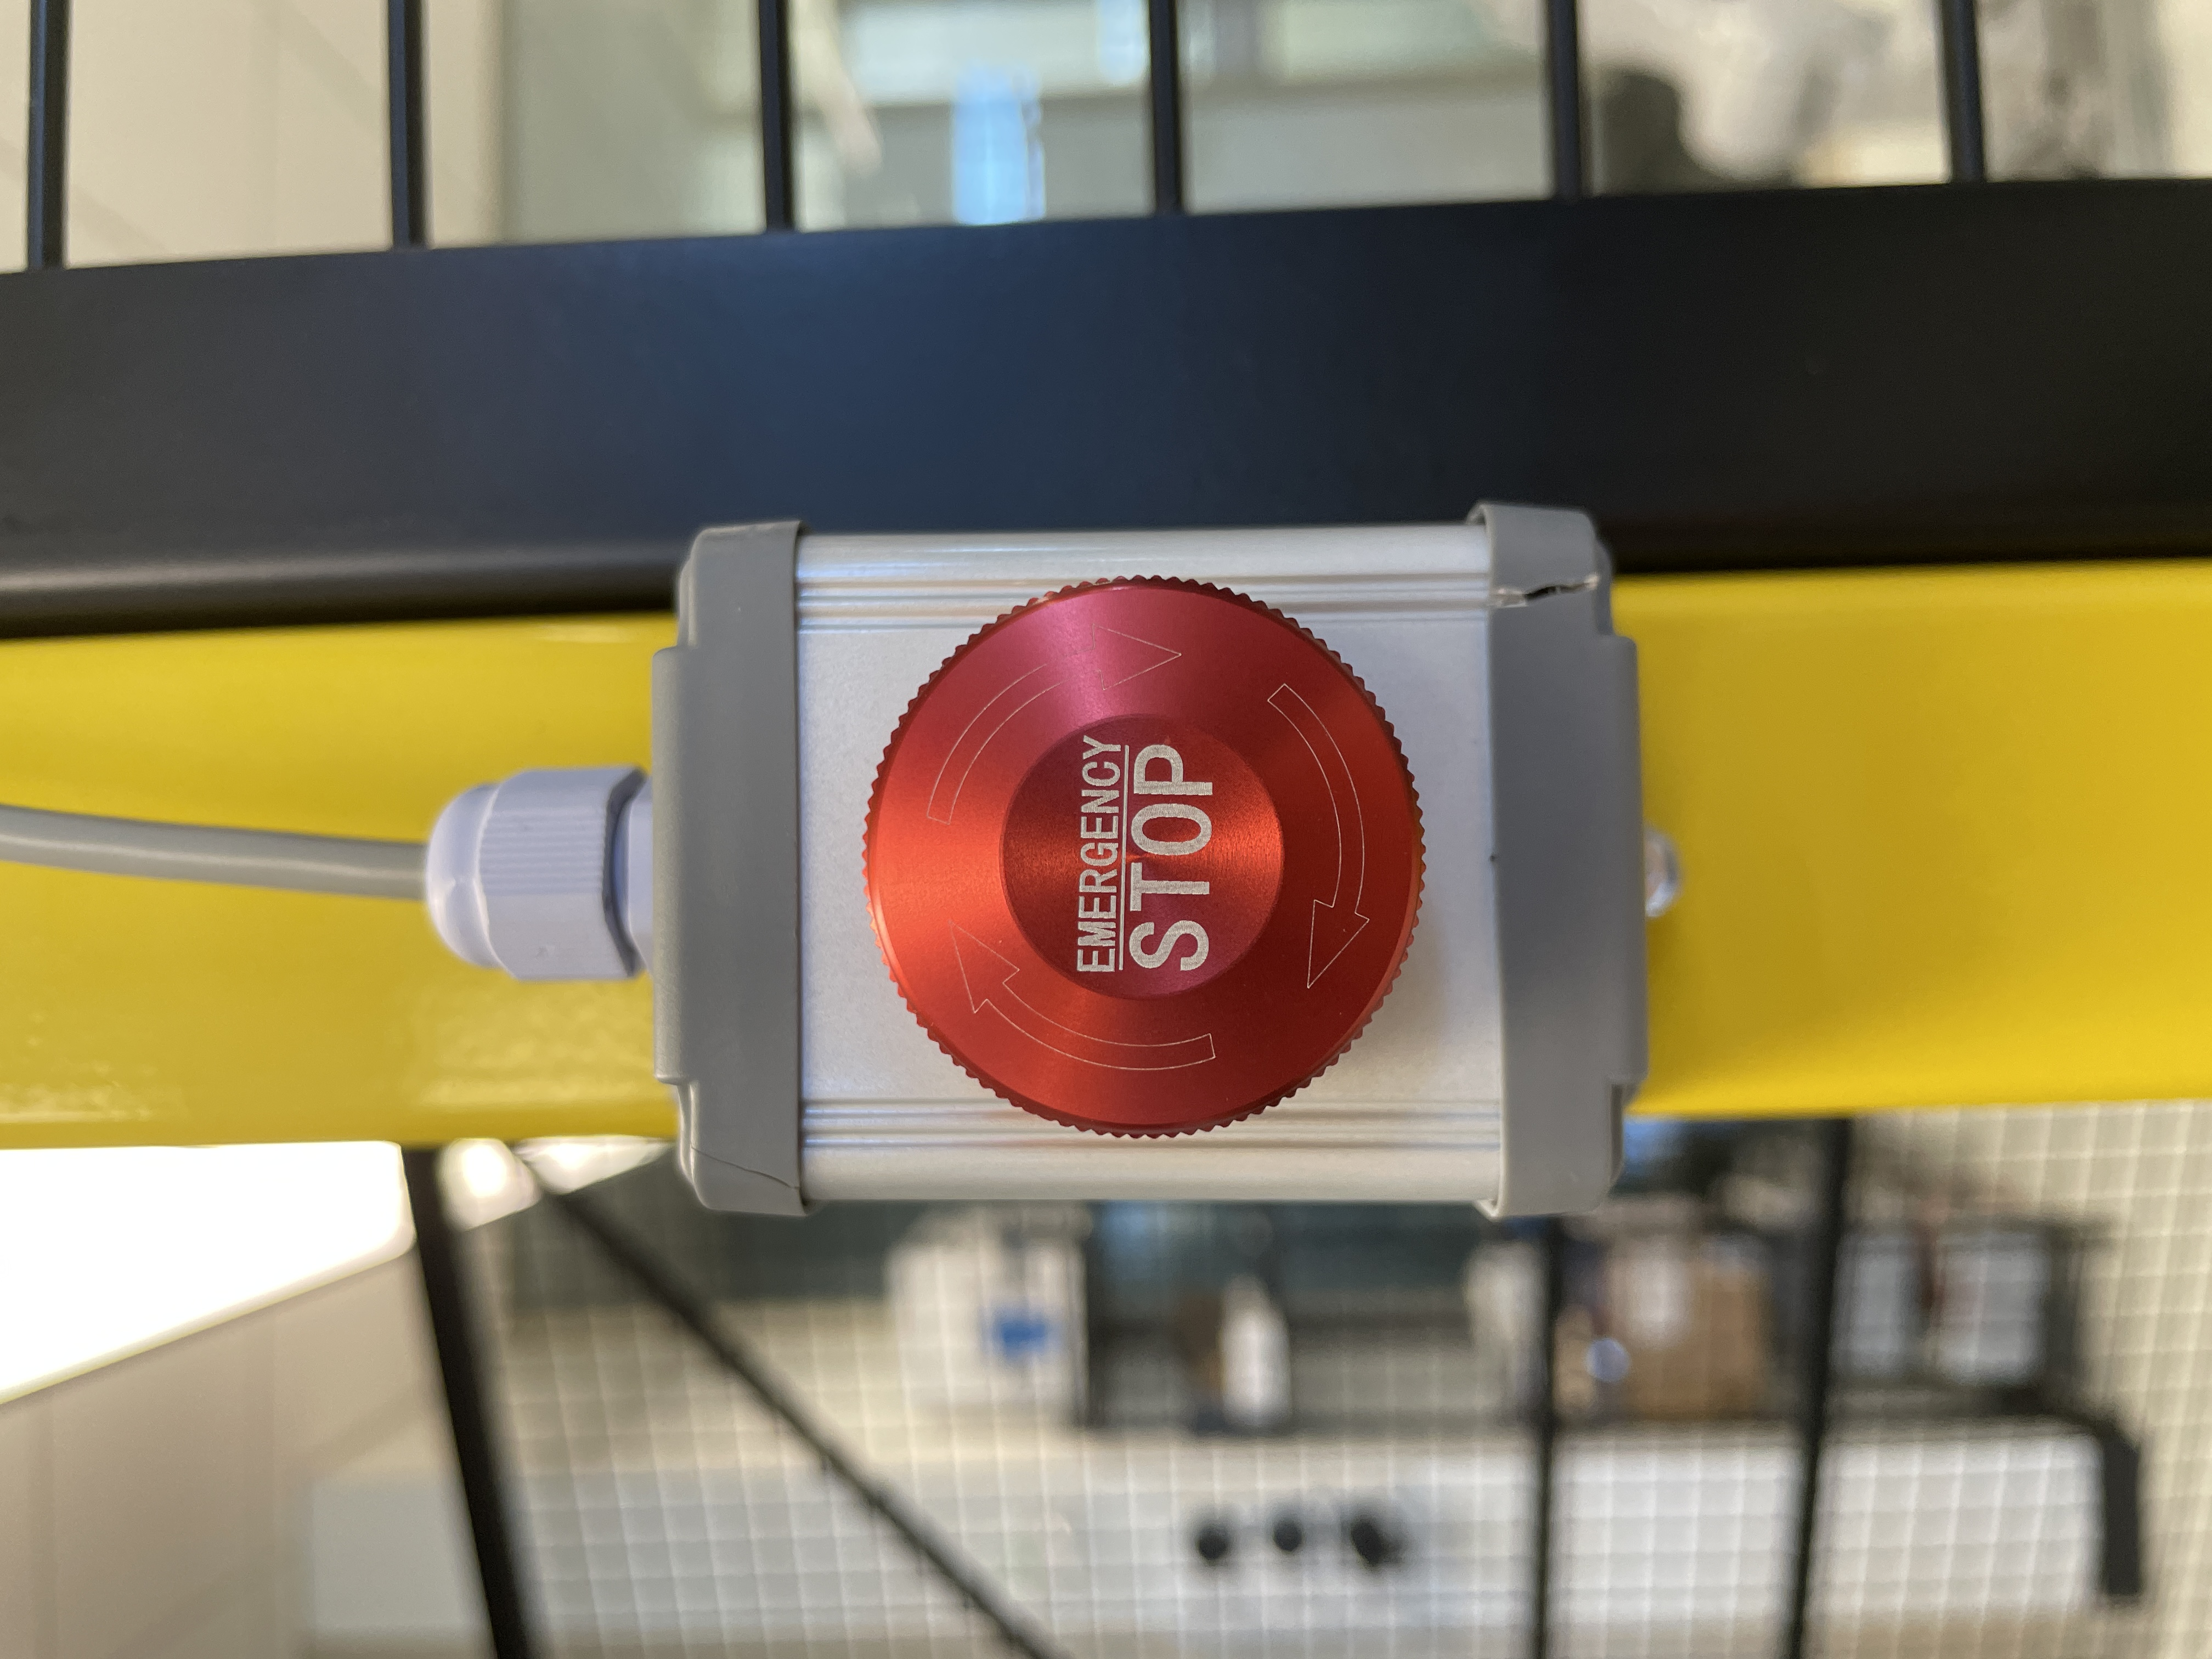
\includegraphics[width=0.40\textwidth, angle = -90]{images/EStop.JPG}
    \caption{Emergency stop}
\end{figure}

\begin{figure}[h!]
	\centering
   	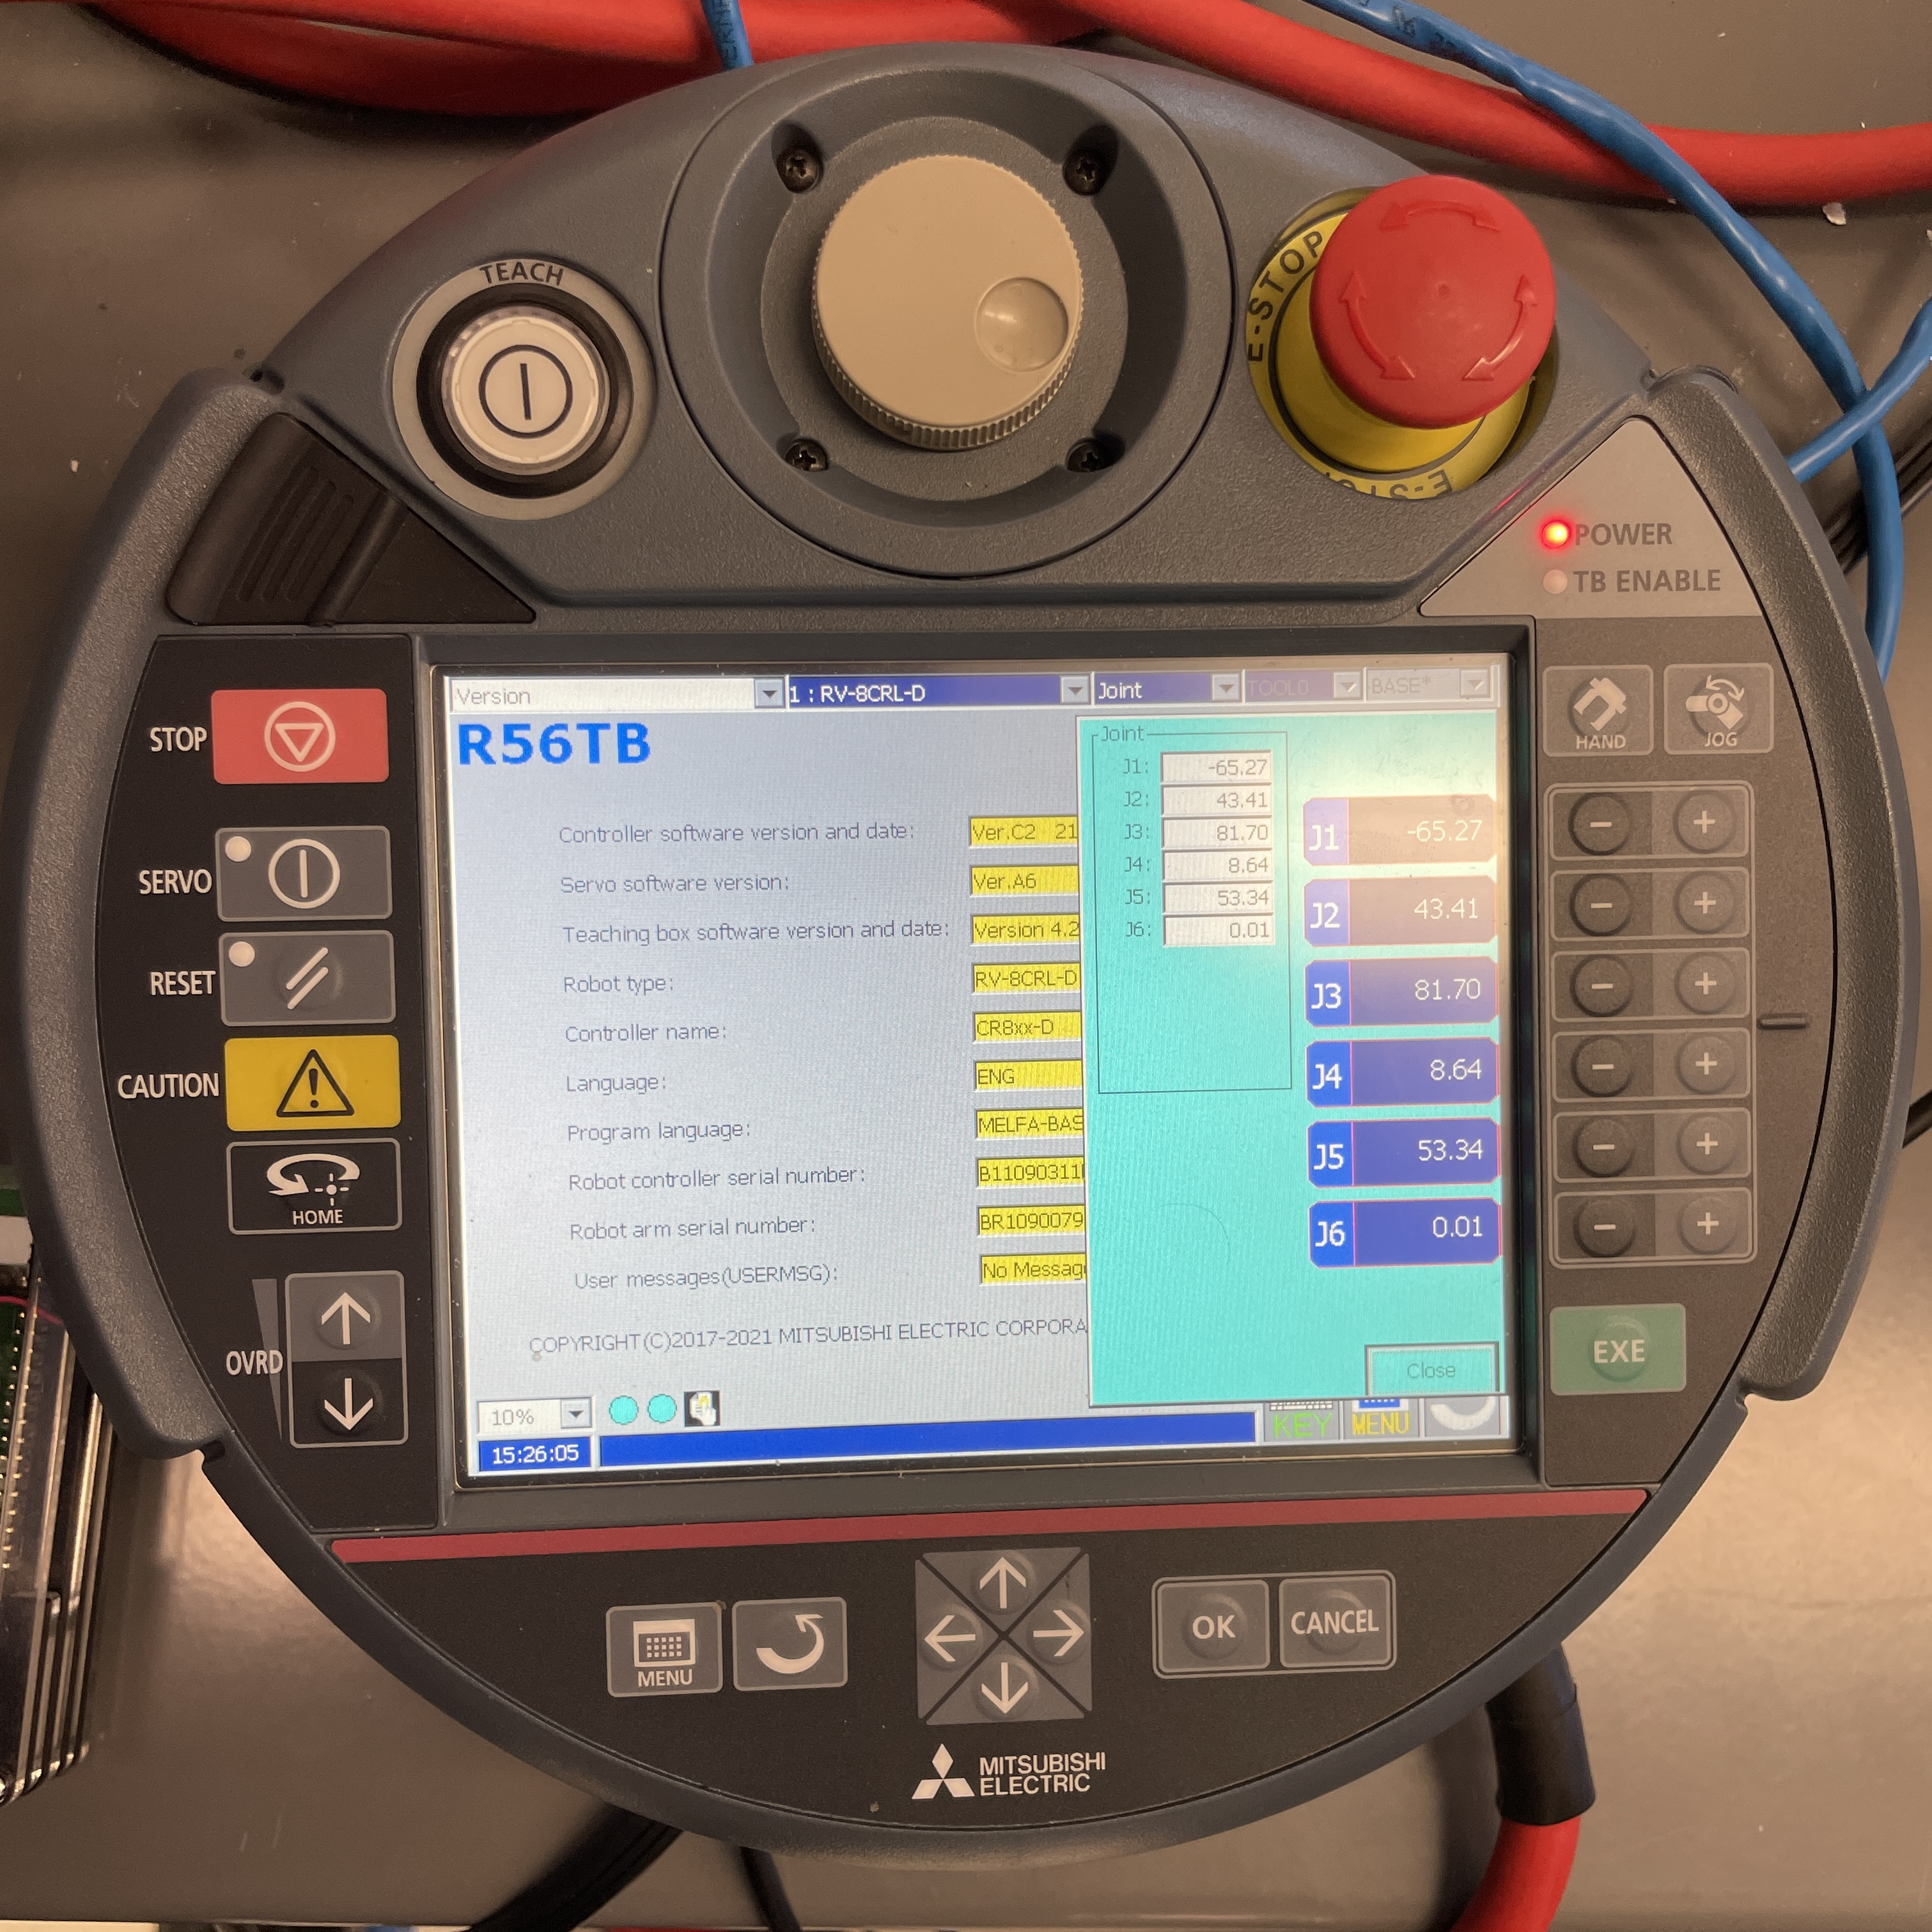
\includegraphics[width=0.40\textwidth]{images/CR800.jpg}
    \caption{CR800 controller}
\end{figure}




\newpage
\section{Customer Requirements}
This project will palletize and depalletize the boxes according to the requirement of the customer defined purpose. The boxes which are less than 7kg in weight will arrange and rearrange the boxes with defined steps as per the operational capacity. This will also implement an extra part to operate functionally for the boxes to keep in required position, QR reader will be implemented. For the safety, the light tower will be implemented to show the operation using different colors.  
\subsection{Barcode reader}
\subsubsection{Description}
By incorporating a QR code or barcode scanner into the RV 8 robot arm, it can be programmed to move to various positions based on the barcode it reads. It can figure out what it is looking at and move accordingly. This means it can neatly stack packages from the ground onto specific rails or take packages off the rail carefully. This scanner helps the robot work better, making it quicker and less likely to make mistakes. It is perfect for jobs where things need to be sorted or moved just right. The RV 8 robot arm can recognize different barcodes, making it really useful for businesses that handle all kinds of stuff.
\subsubsection{Source}
CSE Senior Design project specifications.
\subsubsection{Constraints}
Exceeding weight limitations can lead to performance issues and safety concerns. The budget of the business may limit what can be implemented. The working environment can affect the scanner's performance. Factors like dust, temperature, and humidity might limit its effectiveness and require additional protective measures.
\subsubsection{Standards}
\begin{itemize}
\item ISO/IEC 18004:20xx Information technology - Automatic identification and data capture techniques: The QR code scanner should follow ISO/IEC 18004 for QR code data encoding and data matrix symbols for compatibility and readability.
\item ISO 10218 Robots and robotic devices - Safety requirements for industrial robots: In order to ensure the safe interaction of the robot arm with the QR scanner and other equipment.
\end{itemize}
\subsubsection{Priority}
\begin{itemize}
\item Critical:
The robot's ability to determine its actions and destinations based on QR codes is important. Without this feature, the product would be rendered ineffective.
\end{itemize}
\subsection{Runtime setup}
\subsubsection{Description}
This feature is related to the ability to configure and adjust the time parameters of automated operations or processes within the system. Users can specify the duration of various tasks, ensuring precise control over timing for optimal system performance. This setting allows for the fine-tuning of process duration to meet specific operational needs.
\subsubsection{Source}
Hyun Ho Kim has expressed the need for flexible and customizable runtime settings to adapt the system's performance to their unique requirements. 
\subsubsection{Constraints}
Sustainability: Any changes made to runtime settings should not compromise the system's overall sustainability and energy efficiency.
\subsubsection{Priority}
\begin{itemize}
\item Low:
While the ability to configure runtime parameters is a valuable feature, it is not considered critical to the core functionality of the product at this time.
\end{itemize}
\subsection{Green Light Signal}
\subsubsection{Description}
The green light tower is a visual indicator designed to signal the operational status of a critical system or process. This tower consists of multiple stacked light modules that emit a bright green light when the system is in an operational or "go" status. When the system is in a non-operational or "stop" status, the green light tower remains off. The green light tower serves as a quick and easily visible means of providing real-time status information, enhancing safety and productivity in industrial and manufacturing environments.
\subsubsection{Source}
CSE Senior Design project specifications.
\subsubsection{Constraints}
Health and Safety: It should meet safety standards to prevent potential hazards or misinterpretation of status.
Environmental: The components of the green light tower should be environmentally friendly and compliant with relevant regulations regarding materials and energy consumption.
\subsubsection{Standards}
\begin{itemize}
\item EN ISO 13850: Safety of machinery - Emergency stop function - Principles for design.
\item IEC 60947-5-2:2019 Low-voltage switchgear and controlgear - Part 5-2: Control circuit devices and switching elements - Proximity switches
\end{itemize}
\subsubsection{Priority}
\begin{itemize}
\item High:
This feature is very important for the product as it directly impacts the safety and efficiency of industrial operations. The green light tower is essential for providing real-time status information, enhancing worker safety, and ensuring smooth and error-free processes. Its absence would compromise both operational safety and productivity, making it a fundamental requirement.
\end{itemize}
\subsection{Orange Light Signal}
\subsubsection{Description}
The orange light is a distinctive visual indicator designed to signal specific conditions or events within the system. This light module emits a bright orange light when a predefined condition is met or when a warning or alert status is triggered. It serves as a clear and easily recognizable means of providing immediate visual cues to operators or users, enhancing safety and ensuring efficient response to critical events.
\subsubsection{Source}
CSE Senior Design project specifications.
\subsubsection{Constraints}
Health and Safety: It should meet safety standards to prevent potential hazards or misinterpretation of status.
Environmental: The components of the orange light tower should be environmentally friendly and compliant with relevant regulations regarding materials and energy consumption.
\subsubsection{Standards}
\begin{itemize}
\item EN ISO 13850: Safety of machinery - Emergency stop function - Principles for design.
\item IEC 60947-5-2:2019 Low-voltage switchgear and controlgear - Part 5-2: Control circuit devices and switching elements - Proximity switches
\end{itemize}
\subsubsection{Priority}
\begin{itemize}
\item High:
This feature is very important for the product as it directly impacts the safety and efficiency of industrial operations. The orange light tower is essential for providing real-time status information, enhancing worker safety, and ensuring smooth and error-free processes. Its absence would compromise both operational safety and productivity, making it a fundamental requirement.
\end{itemize}
\subsection{Red Light Signal}
\subsubsection{Description}
The red light signal is a vital visual indicator designed to signal immediate stop or emergency conditions within the system. This light module emits a bright red light when predefined critical events or emergency states occur. It serves as a clear and universally recognized means of conveying urgent visual cues to operators or users, ensuring safety and facilitating quick, decisive responses in emergency situations.
\subsubsection{Source}
CSE Senior Design project specifications.
\subsubsection{Constraints}
Health and Safety: It should meet safety standards to prevent potential hazards or misinterpretation of status.
Environmental: The components of the red light tower should be environmentally friendly and compliant with relevant regulations regarding materials and energy consumption.
\subsubsection{Standards}
\begin{itemize}
\item EN ISO 13850: Safety of machinery - Emergency stop function - Principles for design.
\item IEC 60947-5-2:2019 Low-voltage switchgear and controlgear - Part 5-2: Control circuit devices and switching elements - Proximity switches
\end{itemize}
\subsubsection{Priority}
\begin{itemize}
\item High:
This feature is very important for the product as it directly impacts the safety and efficiency of industrial operations. The red light tower is essential for providing real-time status information, enhancing worker safety, and ensuring smooth and error-free processes. Its absence would compromise both operational safety and productivity, making it a fundamental requirement.
\end{itemize}

\subsection{Palletizing and depalletizing}
\subsubsection{Description}
The main objective of this system is to efficiently arrange and rearrange boxes in a structured manner, sticking to a method specified by the customer. This will be based on the customer's specified method. 
\subsubsection{Source}
Team ROBO CREW 
\subsubsection{Constraints}
In the system design, certain constraints must be considered for functionality. These constraints primarily involve establishing specific offset values that must be configured to align with the desired operational parameters. Before achieving full operational capacity, testing procedures will be necessary to verify and fine-tune these set offset values. These tests will ensure that the system operates within the defined constraints, maintaining accuracy and efficiency in the palletizing and depalletizing processes. 
\subsubsection{Standards}
Not applicable. 
\subsubsection{Priority}
High

\subsection{Installation of Linear Rail}
\subsubsection{Description}
In addition to the robot arm, an important component is required for desire functionality, namely the linear rail. Serving as the system's 7th axis complementing the robot arm's existing 6 axes, the linear rail is a crucial addition. Its primary role is to facilitate backward and forward movements, significantly enhancing the system's versatility. The integration of this linear rail component adds seamless and efficient operations, allowing the robot arm to navigate and position itself with great accuracy and efficiency, meeting the specific customer demands.
\subsubsection{Source}
Team ROBO CREW 
\subsubsection{Constraints}
Linear rail needs to setup properly. 
\subsubsection{Standards}
Not applicable. 
\subsubsection{Priority}
High
\newpage
\section{Packaging Requirements}
Though the RV8-CRL is housed in the Engineering Research Building, this particular project contains several modular hardware and software components components that can be packaged for implementation to other workcells that house the RV8-CRL. This makes it possible to replicate the RV8-CRL's capabilities in other locations, without having to rebuild the entire system from scratch.

\subsection{Hardware components}
\subsubsection{Description}
The hardware components will be placed in a labeled box in the workcell, and will include the gripper, Raspberry Pi, sensors, extra wiring, cardboard boxes, and any other hardware components that are necessary to implement the RV8-CRL project in another working environment. This also will include a USB drive.
\subsubsection{Source}
Dr. Chris McMurrough
\subsubsection{Constraints}
There may be several different wires and hardware components, which can become disorganized if not labeled properly.
\subsubsection{Standards}
There are no applicable standards.
\subsubsection{Priority}
Moderate

\subsection{Software components}
\subsubsection{Description}
All programs, code, scripts, and software will be written to a USB drive, as well as uploaded to a shared version control system GitHub repository.
\subsubsection{Source}
Dr. Chris McMurrough
\subsubsection{Constraints}
The software components must be compatible with the hardware components and operating systems used in the target workcells. Compatibility testing and adjustments may be required to ensure seamless integration.
\subsubsection{Standards}
There are no applicable standards.
\subsubsection{Priority}
Moderate
\newpage
\section{Performance Requirements}
In an industrial setting, the performance and efficiency of machinery are pivotal in determining earnings. Any delay, inefficiency, or downtime in industrial operations can have a direct impact on the profitability of an organization. The RV8-CRL has specific performance requirements to adhere to.

\subsection{Load Capacity}
\subsubsection{Description}
The RV8-CRL has a rated payload of 7 kg (15.432 lbs) and a maximum payload of 8 kg (17.637 lbs).
\subsubsection{Source}
This requirement is sourced by Mitsubishi.
\subsubsection{Constraints}
The gripper used in conjunction with the robot must be designed and configured to support the same payload capacity as specified by the robot's rated and maximum payload. Failure to meet this constraint can lead to suboptimal performance and potential damage to the robot or the objects it handles.
\subsubsection{Standards}
There are no applicable standards.
\subsubsection{Priority}
Critical

\subsection{Positioning with Offset}
\subsubsection{Description}
The RV8-CRL robot must achieve a maximum positioning offset of no more than 1 millimeter (0.039 inches) from the intended target position when performing precision tasks. This requirement ensures that the robot can accurately position objects and perform tasks with a high degree of precision, critical for applications such as assembly, pick-and-place operations, and quality control.
\subsubsection{Source}
This requirement is sourced by industrial robot standard.
\subsubsection{Constraints}
It may be challenging to measure performance accuracy.
\subsubsection{Standards}
ISO 9283 - This standard defines a set of tests for measuring the repeatability, absolute accuracy, and path accuracy of industrial robots
\subsubsection{Priority}
High

\subsection{Positioning with Offset}
\subsubsection{Description}
The RV8-CRL robot must achieve a maximum positioning offset of no more than 1 millimeter (0.039 inches) from the intended target position when performing precision tasks. This requirement ensures that the robot can accurately position objects and perform tasks with a high degree of precision, critical for applications such as assembly, pick-and-place operations, and quality control.
\subsubsection{Source}
This requirement is sourced by industrial robot standard.
\subsubsection{Constraints}
It may be challenging to measure performance accuracy.
\subsubsection{Standards}
ISO 9283 - This standard defines a set of tests for measuring the repeatability, absolute accuracy, and path accuracy of industrial robots
\subsubsection{Priority}
High

\subsection{Box Weight}
\subsubsection{Description}
Boxes used in the demonstration of the RV8-CRL must not exceed a weight of 8 kg (17.637 lbs). This weight limitation is imposed to safeguard the safety of robot operation and to ensure the reliability of its performance. Exceeding this weight may impede structural integrity.
\subsubsection{Source}
This requirement is sourced by industrial robot standard and Mitsubishi.
\subsubsection{Constraints}
This weight limitation restricts the amount of industrial applications that the program can be used in.
\subsubsection{Standards}
ISO 10218-1 and ISO 10218-2:2011 - These international standards provide guidelines for the safety of industrial robots. They include specifications related to the maximum payload and handling of objects by industrial robots.
\subsubsection{Priority}
High
\newpage
\section{Safety Requirements}
The RV-8CRL robot arm is an industrial robot that can potentially harm those around those with electric shocks and serious injuries due to the movement of robot and wiring of robot. We shall include procedures that will make it more safer to be around the robot, and prevent any electrical hazard.

\subsection{Laboratory equipment lockout/tagout (LOTO) procedures}
\subsubsection{Description}
Any fabrication equipment provided used in the development of the project shall be used in accordance with OSHA standard LOTO procedures. Locks and tags are installed on all equipment items that present use hazards, and ONLY the course instructor or designated teaching assistants may remove a lock. All locks will be immediately replaced once the equipment is no longer in use.
\subsubsection{Source}
CSE Senior Design laboratory policy
\subsubsection{Constraints}
Equipment usage, due to lock removal policies, will be limited to availability of the course instructor and designed teaching assistants.
\subsubsection{Standards}
Occupational Safety and Health Standards 1910.147 - The control of hazardous energy (lockout/tagout).
\subsubsection{Priority}
Critical

\subsection{National Electric Code (NEC) wiring compliance}
\subsubsection{Description}
Any electrical wiring must be completed in compliance with all requirements specified in the National Electric Code. This includes wire runs, insulation, grounding, enclosures, over-current protection, and all other specifications.
\subsubsection{Source}
CSE Senior Design laboratory policy
\subsubsection{Constraints}
High voltage power sources, as defined in NFPA 70, will be avoided as much as possible in order to minimize potential hazards.
\subsubsection{Standards}
NFPA 70
\subsubsection{Priority}
Critical

\subsection{RIA robotic manipulator safety standards}
\subsubsection{Description}
Robotic manipulators, if used, will either housed in a compliant lockout cell with all required safety interlocks, or certified as a "collaborative" unit from the manufacturer.
\subsubsection{Source}
CSE Senior Design laboratory policy
\subsubsection{Constraints}
Collaborative robotic manipulators will be preferred over non-collaborative units in order to minimize potential hazards. Sourcing and use of any required safety interlock mechanisms will be the responsibility of the engineering team.
\subsubsection{Standards}
ANSI/RIA R15.06-2012 American National Standard for Industrial Robots and Robot Systems, RIA TR15.606-2016 Collaborative Robots
\subsubsection{Priority}
Critical

\subsection{Emergency Stop}
\subsubsection{Description}
Robotic arm manipulator shall stop once any of the exterior, interior, and controller emergency stops are pressed.
\subsubsection{Source}
CSE Senior Design laboratory policy
\subsubsection{Constraints}
Only 2 emergency stops will be provided that are located outside the controller. Additionally, only those allowed to enter the work cell, instructor and the engineering team, shall have access to the interior and controller emergency stop.
\subsubsection{Standards}
RV-8CRL Standards Specification
\subsubsection{Priority}
Critical

\subsection{Inductive Switch}
\subsubsection{Description}
Since the linear rail has bounds, inductive switches shall be used to prevent the robot arm from going beyond a certain limits. These inductive swtiches will be added on both ends of the linear rail.
\subsubsection{Source}
CSE Senior Design RV8 Engineering Team
\subsubsection{Constraints}
The inductive switches will only work if they are programmed into stopping the robot arm. Otherwise, they won't prevent the robot arm from traveling beyond those limits.
\subsubsection{Standards}
There are no applicable standards.
\subsubsection{Priority}
Critical

\newpage
\section{Maintenance \& Support Requirements}
Apart from customers' requirements the team will provide to ensure robot performs smoothly. 
\subsection{Operation Manual}
\subsubsection{Description}
A detailed operation manual will be provided to the customer. It will guide the customer through various steps to operate the robot. This will include the start, stop and any kind of minor malfunctioning troubleshoot procedures.  
\subsubsection{Source}
Team ROBO CREW 
\subsubsection{Constraints}
A manual should be followed accurately and should ask for assistance if needed in understanding. \subsubsection{Standards}
No applicable standards. 
\subsubsection{Priority}
Medium to high.

\subsection{Safety Connections}
\subsubsection{Description}
The team will assist by providing appropriate safety connections which include E-stops, industrial light towers, and inductive sensors, since this is an industry standard robot it requires 2 E-stops and a light tower. The light tower lights will indicate the current mode of the robot. E-stops will be placed in and out of the facility where the robot is operational. 
\subsubsection{Source}
Team ROBO CREW 
\subsubsection{Constraints}
The customer needs to follow safety procedures as instructed. 
\subsubsection{Standards}
OSHA standards 
\subsubsection{Priority}
High.

\subsection{Major Connections}
\subsubsection{Description}
There are several components which will require the connection between them. The team will assist with the connection between PLC, Controller, and PC which will be used to operate this robot arm. The other connections will be the air compressor which will help operate the airbrush attached to the arm. \subsubsection{Source}
Team ROBO CREW 
\subsubsection{Constraints}
No constraints.
\subsubsection{Standards}
No applicable standards. 
\subsubsection{Priority}
High.
\newpage
\section{Other Requirements}
Include a header paragraph specific to your product here. In this section specify anything else that is required for the product to be deemed complete. Include requirements related to customer setup and configuration if not specified in a previous requirement. Add any known requirements related to product architecture/design, such as modularity, extensibility (for future enhancements), or adaptation for a specific programming language. Consider requirements such as portability of your source code to various platforms (Windows, Linux, Unix Mac OS, etc.).

\subsection{Host PC Security}
\subsubsection{Description}
The PC that is hosting the robot and the robot controllers must be secure with a username and password authentication.\subsubsection{Source}
UTA Senior Design.
\subsubsection{Constraints}
The login information must be passed down to future teams.
\subsubsection{Standards}
There are no applicable standards.
\subsubsection{Priority}
Moderate
\newpage
\section{Future Items}
Possible improvements to this project include the graphical user interface with a user who can control the movements using simple data. This will be implemented if everything goes well before the schedule.  
\subsection{GUI App}
\subsubsection{Description}
A future item which can be added to this project is to provide the customer with GUI application. This will give all the options on graphical user interface. 
\subsubsection{Source}
Team ROBO CREW.
\subsubsection{Constraints}
Good hands-on training will be required using the GUI application. 
\subsubsection{Standards}
Not applicable.  
\subsubsection{Priority}
Low.
\newpage

%%% References
\bibliographystyle{plain}
\bibliographystyle{reference/IEEEtran_custom}
\bibliography{reference/refs}{}

\end{document}